\documentclass[a4paper,12pt]{article}
\usepackage[utf8]{vietnam}
\usepackage{geometry}
\usepackage{graphicx}
\usepackage{amsmath}
\usepackage{titlesec}
\usepackage{tikz}
\usepackage{enumitem}
\usepackage{fancyvrb}
\usepackage{tocloft}
\usepackage[hidelinks]{hyperref}
\usepackage{etoolbox}
\usepackage{float}
\usepackage{xcolor}

\definecolor{color}{rgb}{0.4, 0.4, 0.4}

\geometry{a4paper, margin=1in}
\pagestyle{plain}

\begin{document}

\begin{tikzpicture}[remember picture, overlay]
    \draw[line width=3pt] ([shift={(1cm,1cm)}]current page.south west) rectangle ([shift={(-1cm,-1cm)}]current page.north east);
    \draw[line width=1pt] ([shift={(1.1cm,1.1cm)}]current page.south west) rectangle ([shift={(-1.1cm,-1.1cm)}]current page.north east);
\end{tikzpicture}

\begin{center}

    {\Large \textbf{POSTS AND TELECOMMUNICATIONS INSTITUTE OF TECHNOLOGY}} \\
    \vspace{0.2cm}
    {\small UNIT: INFORMATION TECHNOLOGY} \\
    \vspace{0.5cm}
    
    
\includegraphics[width=0.4\textwidth]{images/logo.png} \\
    \vspace{0.5cm}
    
    {\Large \textbf{ASSIGNMENT REPORT}} \\
    \vspace{0.2cm}
    {\large \textbf{SUBJECT: PYTHON}} \\
    \vspace{1.5cm}
    
    \begin{center}
    \begin{tabular}{ll}
    \vspace{0.3cm}
    
    \textbf{LECTURER} & : Kim Ngoc Bach \\
    \vspace{0.3cm}
    
    \textbf{CLASS} & : B23CQCE04-B\\
    \vspace{0.3cm}
    
    \textbf{STUDENTS} & : Pham Quang Vinh - B23DCCE100\\
    & \ \ Do Tien Thanh - B23DCCE239
    \end{tabular}
    \end{center}
\end{center}
\newpage

\renewcommand{\figurename}{Image}

\renewcommand{\contentsname}{Contents}

\setlength{\cftbeforesecskip}{12pt}       
\setlength{\cftbeforesubsecskip}{8pt}     

\setlength{\cftbeforesecskip}{20pt}
\setlength{\cftbeforesubsecskip}{12pt}

{\large
\tableofcontents
}
\newpage

\section{Requirements}
\begin{itemize}
    \item Classify images from CIFAR-10 dataset with following tasks:
    \begin{itemize}[label= -]
        \item Build a basic MLP (Multi-Layer Perceptron) neural network with 3 layers.
        \item Build a CNN (Convolutional Neural Network) with 3 convolution layers.
        \item Perform image classification using both neural networks, including training, validation,
        \item and testing.
        \item Plot learning curves.
        \item Plot confusion matrix.
        \item Compare and discuss the results of the two neural networks.
        \item Use the PyTorch library.
    \end{itemize}

    \item With these tasks above, we need to install some necessary libraries:
    \begin{itemize}[label= -]
        \item \textbf{torch}: Core PyTorch library for tensor operations.
        \item \textbf{torchvision}: Provides datasets (e.g., CIFAR-10) and image tranformation utilities.
        \item \textbf{matplotlib}: For plotting training curves.
        \item \textbf{numpy}: for numerical operations.
        \item \textbf{scikit-learn}: For deep learning.
        \item \textbf{seaborn}: For visualizing confusion matrices as heatmaps.
    \end{itemize}
\end{itemize}
\newpage 

\section{Solutions}
\subsection{Setup and preprocessing}
\begin{itemize}
    \item \textbf{Set random seed}:
    \begin{Verbatim}[xleftmargin=-1cm]
        torch.manual_seed(42)
    \end{Verbatim}
    \begin{itemize}
        \item We set a random seed for reproducibility, ensuring consistent random number generation (e.g., for weight initialization).
    \end{itemize}

    \item \textbf{Device setup}:
    \begin{Verbatim}[xleftmargin=-1cm]
        device = torch.device("cuda" if torch.cuda.is_available() else "cpu")
    \end{Verbatim}
    \begin{itemize}
        \item Checks if a GPU is available (\textit{cuda}). If not, it defaults to the CPU. Models and data will be moved to this device for computation.

        \item Priority use GPU for training images classification model because it improve the training time, able to train complex model like the CNN without excessive delays.
    \end{itemize}

    \item \textbf{Data loading and preprocessing}:
    The code loads the CIFAR-10 dataset and prepares it for training and testing.
    \begin{itemize}
        \item Transformations:
        \begin{Verbatim}[xleftmargin=-1cm]
            transform = transforms.Compose([
                transforms.ToTensor(),
                transforms.Normalize((0.5, 0.5, 0.5), (0.5, 0.5, 0.5))
            ])
        \end{Verbatim}  
        \begin{itemize}
            \item \textbf{transforms.ToTensor()}: Converts images to PyTorch tensors with shape (C, H, W) and scales pixel values from [0, 255] to [0, 1].

            \item \textbf{transforms.Normalize((0.5, 0.5, 0.5), (0.5, 0.5, 0.5))}: Normalizies the RGB channels to have a mean of 0.5 and standard deviation of 0.5, resulting in values roughly in [-1, 1]. This helps stabilize training.
        \end{itemize}

        \item Loading CIFAR-10 Dataset:
        \begin{Verbatim}[xleftmargin= -2cm]  
        
            trainset = torchvision.datasets.CIFAR10(root='./SourceCode/data', 
                        train=True,download=True, transform=transform)
            trainloader = torch.utils.data.DataLoader(trainset, batch_size=64,
                        shuffle=True, num_workers=2)
            testset = torchvision.datasets.CIFAR10(root='./SourceCode/data', 
                        train=False, download=True, transform=transform)
            testloader = torch.utils.data.DataLoader(testset, batch_size=64,
                        shuffle=False, num_workers=2)
                        
        \end{Verbatim}  
        The CIFAR-10 dataset consists of 60,000 32×32 color (RGB) images divided into 10 classes, such as airplane, car, and bird. Out of the total images, 50,000 are used for training and 10,000 for testing.
        
        The parameter \verb|root='./SourceCode/data'| specifies the directory where the dataset will be stored or downloaded. The \verb|train=True| or \verb|train=False| flag selects whether to load the training or test split, respectively. Setting \verb|download=True| allows the dataset to be downloaded automatically if it is not already available in the specified directory.
        
        To handle the data efficiently, the dataset is wrapped using a \textbf{DataLoader}, which enables batching and optional shuffling of the data. The \verb|batch_size=64| setting means that data will be processed in batches of 64 images. During training, \verb|shuffle=True| is used to randomize the order of the training samples, which helps prevent the model from overfitting to the sequence of the data. In contrast, \verb|shuffle=False| is used during testing to ensure consistent evaluation.
        
        Finally, \verb|num_workers=2| configures the DataLoader to use two subprocesses for loading the data in parallel, which can significantly speed up data retrieval.

        Defines the 10 CIFAR-10 class labels for reference in visualization like 'plane', 'car', 'bird', ...
    \end{itemize}
\end{itemize}

\subsection{Build a basic MLP (Multi-Layer Perceptron) neural network with 3 layers}

\begin{figure}[h]
    \centering
    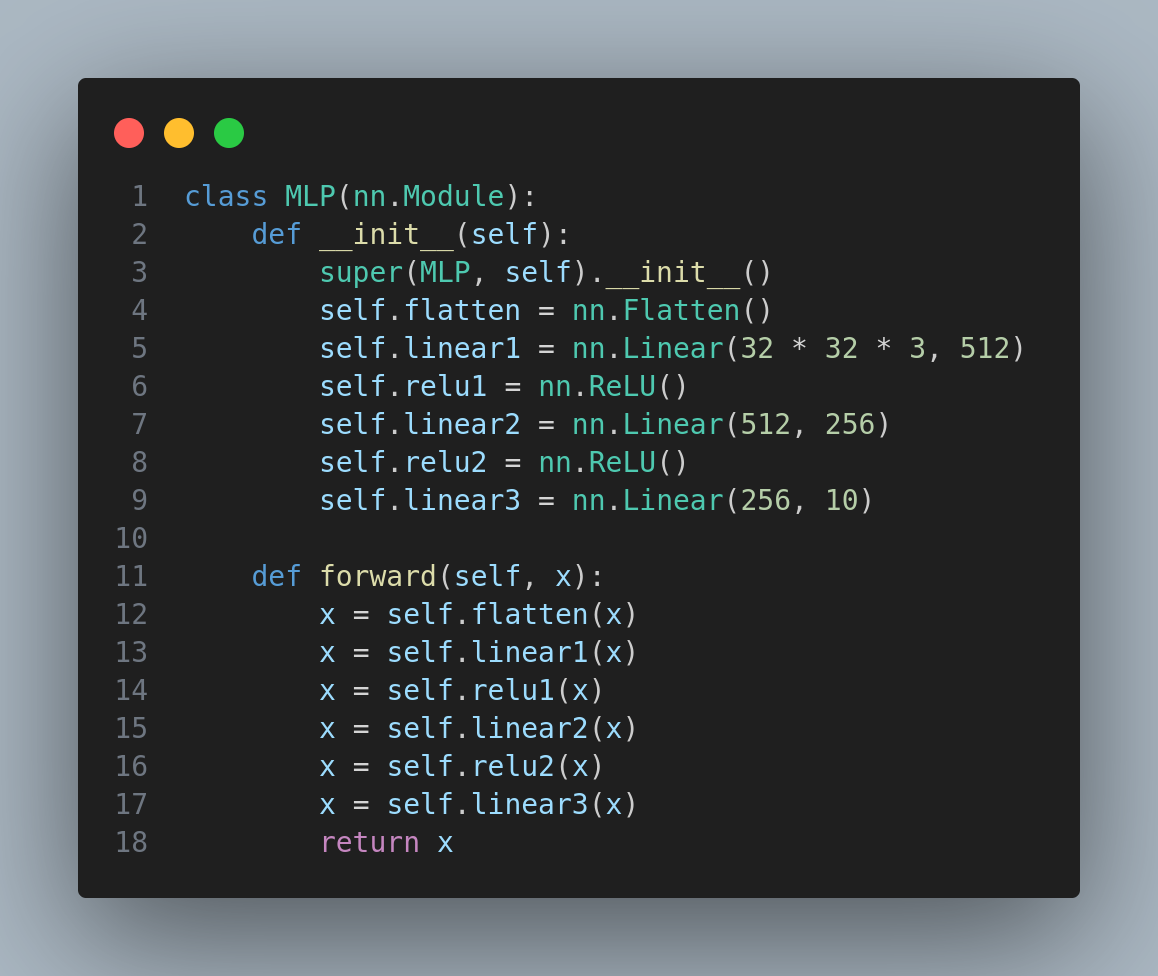
\includegraphics[width=0.7\linewidth]{images/MLP_model.png}
    \label{fig:enter-label}
\end{figure}

\begin{itemize}
    \item \textbf{Class Definition}
    \begin{itemize}
        \item The \textbf{MLP} class defines a multilayer perceptron (MLP) neural network designed for image classification on the CIFAR-10 dataset. It inherits from \verb|nn.Module|, which is the base class for all neural network models in PyTorch. By inheriting from this class, the \textbf{MLP} model gains all the functionality needed to define layers, manage parameters, and perform forward computations.
    \end{itemize}

    \item \textbf{Initialization}
    \begin{itemize}
        \item In the constructor (\verb|__init__| method), the model begins by calling \verb|super(MLP,| \verb|self).__init__()| to properly initialize the parent \verb|nn.Module| class. The model then defines its architecture layer by layer. First, it includes a flattening layer, \verb|nn.Flatten()|, which reshapes the input image from its original shape of \verb|[batch_size, 3, 32, 32]| into a flat vector of size \verb|[batch_size, 3072]|, where 3072 corresponds to 3 (channels) × 32 (height) × 32 (width). This transformation is necessary because fully connected layers expect 2D input with shape \verb|[batch_size, features]|.

        \item Next, the model defines three fully connected (linear) layers with ReLU activation functions in between. The first linear layer maps the 3072 input features to 512 hidden units using \verb|nn.Linear(32 * 32 * 3, 512)|. A ReLU activation, \verb|nn.ReLU()|, follows to introduce non-linearity. The second linear layer reduces the 512 features down to 256 units, again followed by another ReLU activation. Finally, the third linear layer maps the 256 hidden units to 10 output units, one for each class in the CIFAR-10 dataset. This final output does not include a softmax, as it typically outputs raw logits, which are then processed by a loss function like cross-entropy during training.
    \end{itemize}

    \item \textbf{Forward Pass}
    \begin{itemize}
        \item The forward method defines the forward pass of the model—that is, how data flows through the network during computation. Input images are first flattened, then passed sequentially through the first linear layer and ReLU, followed by the second linear layer and ReLU, and finally through the third linear layer. The resulting output is a vector of 10 logits representing the model's unnormalized confidence scores for each CIFAR-10 class.
    \end{itemize}

    In summary, this class encapsulates a simple yet effective MLP architecture for image classification, converting raw image data into class scores through a series of fully connected layers and non-linear activations.
\end{itemize}
\newpage

\subsection{Build a CNN (Convolutional Neural Network) with 3 convolution layers.}

\begin{figure}[h]
    \centering
    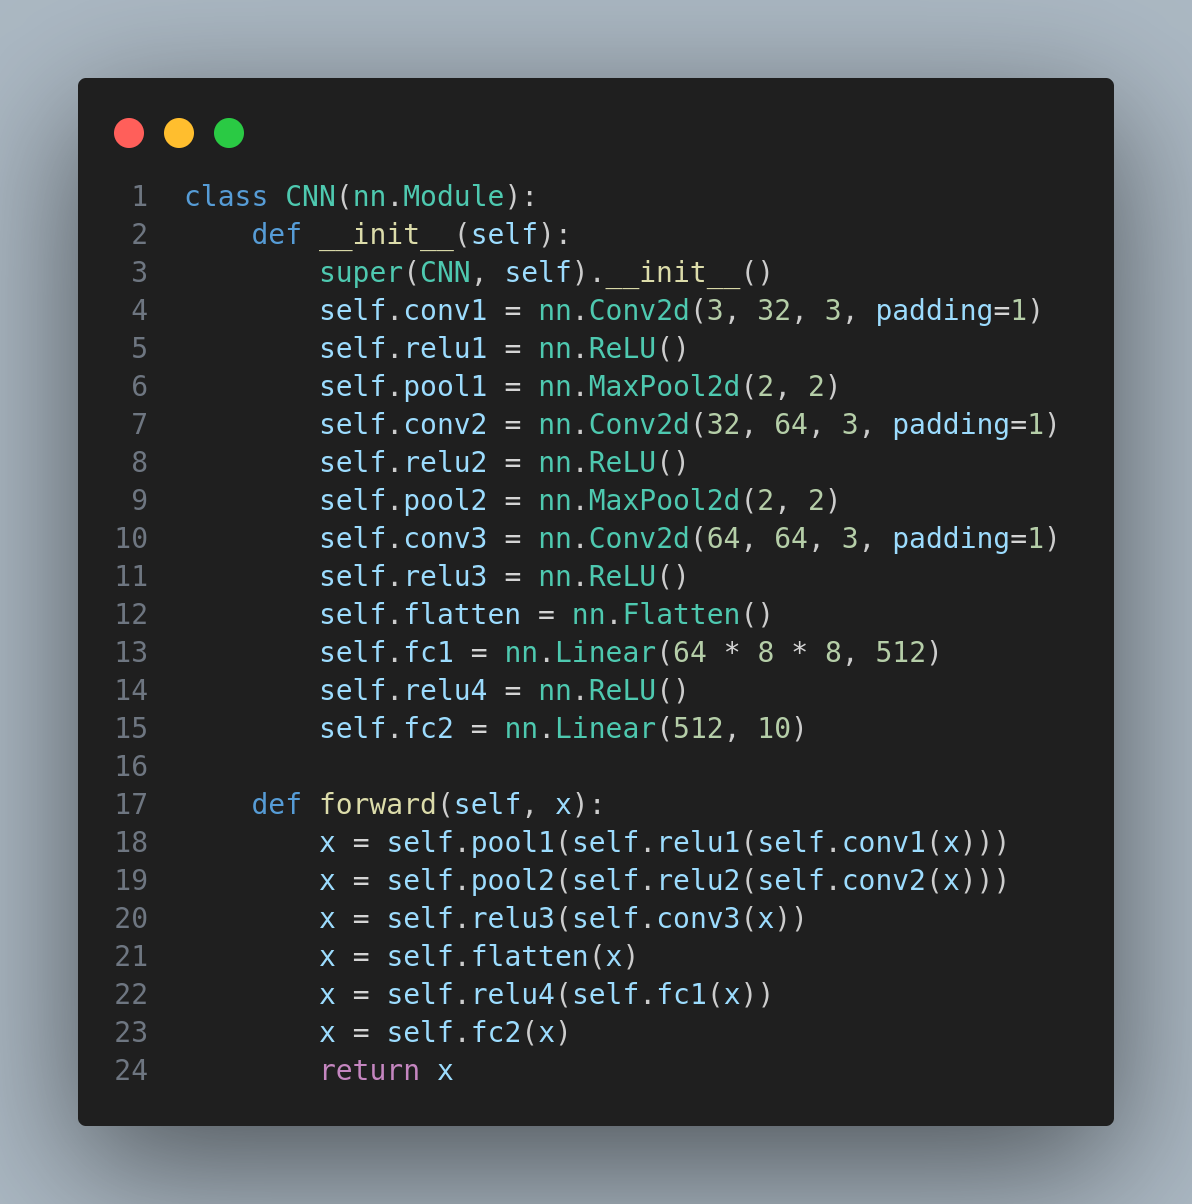
\includegraphics[width=0.6\linewidth]{images/CNN_model.png}
    \caption{CNN Model}
    \label{fig:enter-label}
\end{figure}

\begin{itemize}
    \item \textbf{Class Definition}
    \begin{itemize}
        \item We define our convolutional neural network (CNN) model using a custom \textbf{CNN} class that inherits from PyTorch’s \verb|nn.Module|. This inheritance allows us to leverage PyTorch’s powerful features, such as automatic gradient tracking, device management (e.g., \verb|.to(device)| for moving models between CPU and GPU), and support for training and evaluation modes. Within the class constructor, we call \verb|super(CNN,| \verb|self).__init__()| to properly initialize the parent class, which sets up the necessary internal structures for PyTorch modules.
    \end{itemize}

    \item \textbf{Initialization}
    \begin{itemize}
        \item In the \verb|__init__| method, we define all layers of the CNN as attributes of the class. These include convolutional layers, activation functions, pooling layers, flattening, and fully connected layers. The first convolutional layer, \verb|self.conv1 = nn.Conv2d(3, 32, 3, padding=1)|, takes in 3-channel RGB images (as in the CIFAR-10 dataset), and applies 32 filters of size 3×3. The padding ensures that the spatial dimensions of the output match the input (32×32 pixels). This layer is responsible for learning low-level features such as edges and textures.

        \item Following this, the second convolutional layer \verb|self.conv2 = nn.Conv2d(32,| \verb| 64, 3, padding=1)| increases the number of output channels to 64, enabling the model to capture more complex features by combining those from the previous layer. Similarly, the third convolutional layer, \verb|self.conv3 = nn.Conv2d(64,| \verb| 64, 3, padding=1)|, retains the same number of channels but refines the learned features. Each convolutional layer is followed by a ReLU activation function, which introduces non-linearity and helps the model learn complex mappings.
        
        \item We also include two max-pooling layers (\verb|self.pool1| and \verb|self.pool2|), which reduce the spatial dimensions by half using a 2×2 kernel and a stride of 2. This not only reduces computational cost but also improves the model’s robustness to small shifts in the input. After the second pooling operation, the feature map size is reduced to 64 channels of 8×8 pixels.
        
        \item To prepare the data for the fully connected layers, we flatten the feature maps using \verb|nn.Flatten()|, converting the [batch, 64, 8, 8] tensors into [batch, 4096] vectors. The first fully connected layer, \verb|self.fc1 = nn.Linear(4096, 512)|, reduces this vector to 512 dimensions. We apply another ReLU activation afterward to maintain non-linearity. Finally, \verb|self.fc2 = nn.Linear(512, 10)| outputs the final logits, one for each of the ten CIFAR-10 classes.
    \end{itemize}

    \item \textbf{Forward pass}
    \begin{itemize}
        \item The forward method defines the actual data flow through the model. The input passes through the convolutional layers with ReLU activations and pooling in sequence, followed by the third convolution and ReLU without pooling. We then flatten the output and apply the fully connected layers to obtain the final logits. The model input is a batch of RGB images of shape [batch, 3, 32, 32], and the output is a tensor of shape [batch, 10], representing the unnormalized scores for each class.
    \end{itemize}

    We use this CNN model in our training pipeline by instantiating it with cnn = CNN().to(device), where device could be a CPU or GPU. The model is optimized using the Adam optimizer with a learning rate of 0.001. Training and evaluation are conducted using the train\_model and evaluate\_model functions, which process batches of CIFAR-10 images through the network.

    Overall, this CNN architecture is well-suited for image classification tasks. It outperforms MLPs in both accuracy and efficiency by maintaining spatial information through convolution and pooling. While a simple MLP might achieve 50–60% accuracy on CIFAR-10, our CNN can reach 70–80% with proper training. The combination of convolutional feature extraction and fully connected classification makes it an effective model for visual recognition problems.
\end{itemize}
\newpage

\subsection{Perform image classification using both neural network}
First of all, to train two models, we wrote the \textbf{train\_model} function for reuse purpose.

\begin{figure}
    \centering
    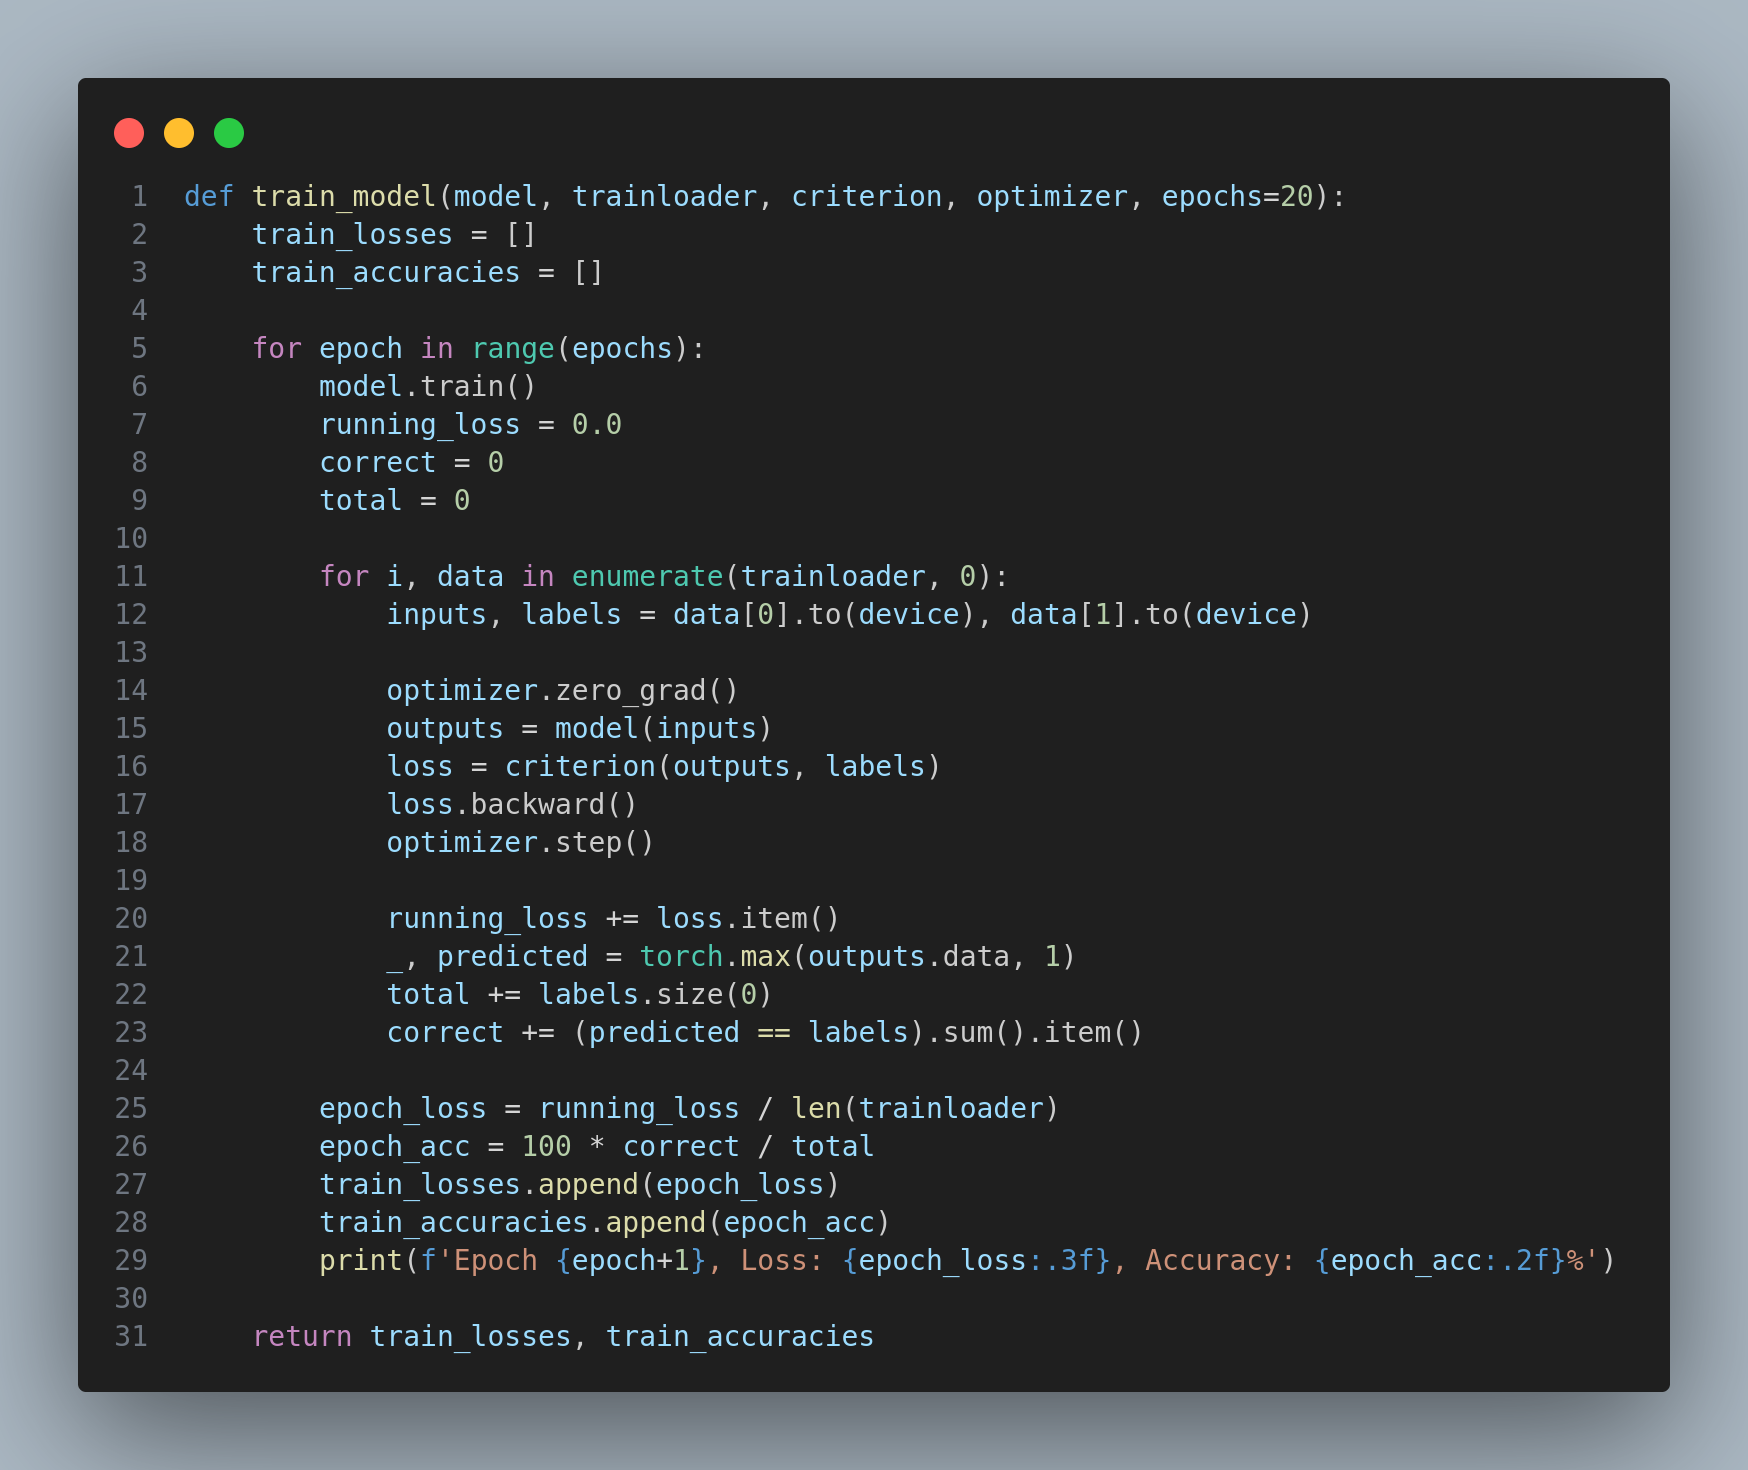
\includegraphics[width=0.7\linewidth]{images/train_func.png}
    \caption{Training function}
    \label{fig:enter-label}
\end{figure}

\begin{itemize}
    \item \textbf{Purpose}
    \begin{itemize}
        \item The purpose of the \verb|train_model| function is to train a neural network—either an MLP or a CNN—on the CIFAR-10 training dataset by optimizing its parameters to minimize classification error. This function processes the training data in batches, applies backpropagation to update the model's weights, and tracks key performance metrics such as training loss and accuracy across multiple epochs.
    \end{itemize}

    \item \textbf{Input(Arguments)}
    \begin{itemize}
        \item This function accepts several inputs. The first is \verb|model|, which refers to the neural network to be trained. This could be either a multi-layer perceptron (MLP) or a convolutional neural network (CNN), both of which are subclasses of \verb|nn.Module| in PyTorch. 
        
        \item  The second input is \verb|trainloader|, a PyTorch \verb|DataLoader| that provides batches of training data. For CIFAR-10, the training set consists of 50,000 images, and we typically use a batch size of 64. The \verb|criterion| is the loss function—specifically, \verb|nn.CrossEntropyLoss()|—which computes the discrepancy between the predicted class scores (logits) and the true labels. 
        
        \item The \verb|optimizer|, such as \verb|optim.Adam(model.parameters()|, lr=0.001), adjusts the model’s weights to minimize the loss function. Finally, we set \verb|epochs=20| by default, meaning the model will see the entire training dataset 20 times.
    \end{itemize}

    \item \textbf{Training process}
    \begin{itemize}
        \item The function begins by initializing two empty lists, \verb|train_losses| and \\ \verb|train_accuracies|, which will store the average loss and accuracy for each epoch. These metrics help us monitor training progress and are typically used to plot learning curves.

        \item We then enter a loop that iterates over the number of epochs. For each epoch, we first set the model to training mode by calling \verb|model.train()|. This ensures that certain layers like dropout or batch normalization behave correctly during training (even though our current model doesn’t include them). We then iterate over the training data in batches using a \textbf{for} loop. Each batch consists of a tuple: \verb|data[0]| contains the input images, shaped as \verb|[batch_size, 3, 32, 32]|, and \verb|data[1]| contains the labels, shaped as \verb|[batch_size]|. We move both the inputs and labels to the appropriate device (CPU or GPU) using \verb|.to(device)|.
        
        \item Next, we perform the forward pass. We begin by resetting the gradients with \verb|optimizer.zero_grad()| to prevent gradient accumulation from previous iterations. Then we pass the inputs through the model to get the output logits: \verb|outputs = model(inputs)|. We compute the loss using \verb|criterion(outputs,| \verb|labels)|, which calculates how far the predicted logits are from the true labels.
        
        \item In the backward pass, we compute gradients with \verb|loss.backward()| and then call \verb|optimizer.step()| to update the model parameters based on those gradients. This process adjusts the model to better predict the correct classes over time.
        
        \item We also track training metrics for each batch. The batch loss is accumulated with \verb|running_loss += loss.item()|. We then use \verb|torch.max(outputs.data, 1)| to get the predicted class indices for each image, and we compare these with the true labels to count the number of correct predictions. These values are accumulated across the epoch.
        
        \item At the end of each epoch, we compute the average loss as \verb|epoch_loss = | \\ \verb|running_loss / len(trainloader)| and the accuracy as \verb|epoch_acc = 100 * | \\ \verb|correct / total|. We store these values in the \verb|train_losses| and \verb|train_accuracies| lists, respectively, and print a summary of the epoch’s performance using a formatted string.
        
        \item Finally, the function returns the lists \verb|train_losses| and \verb|train_accuracies|, each containing 20 values corresponding to the 20 training epochs.
    \end{itemize}
    
\end{itemize}
\newpage

Second, is evaluation, we also wrote the \textbf{evaluate\_model}

\begin{figure}[h]
    \centering
    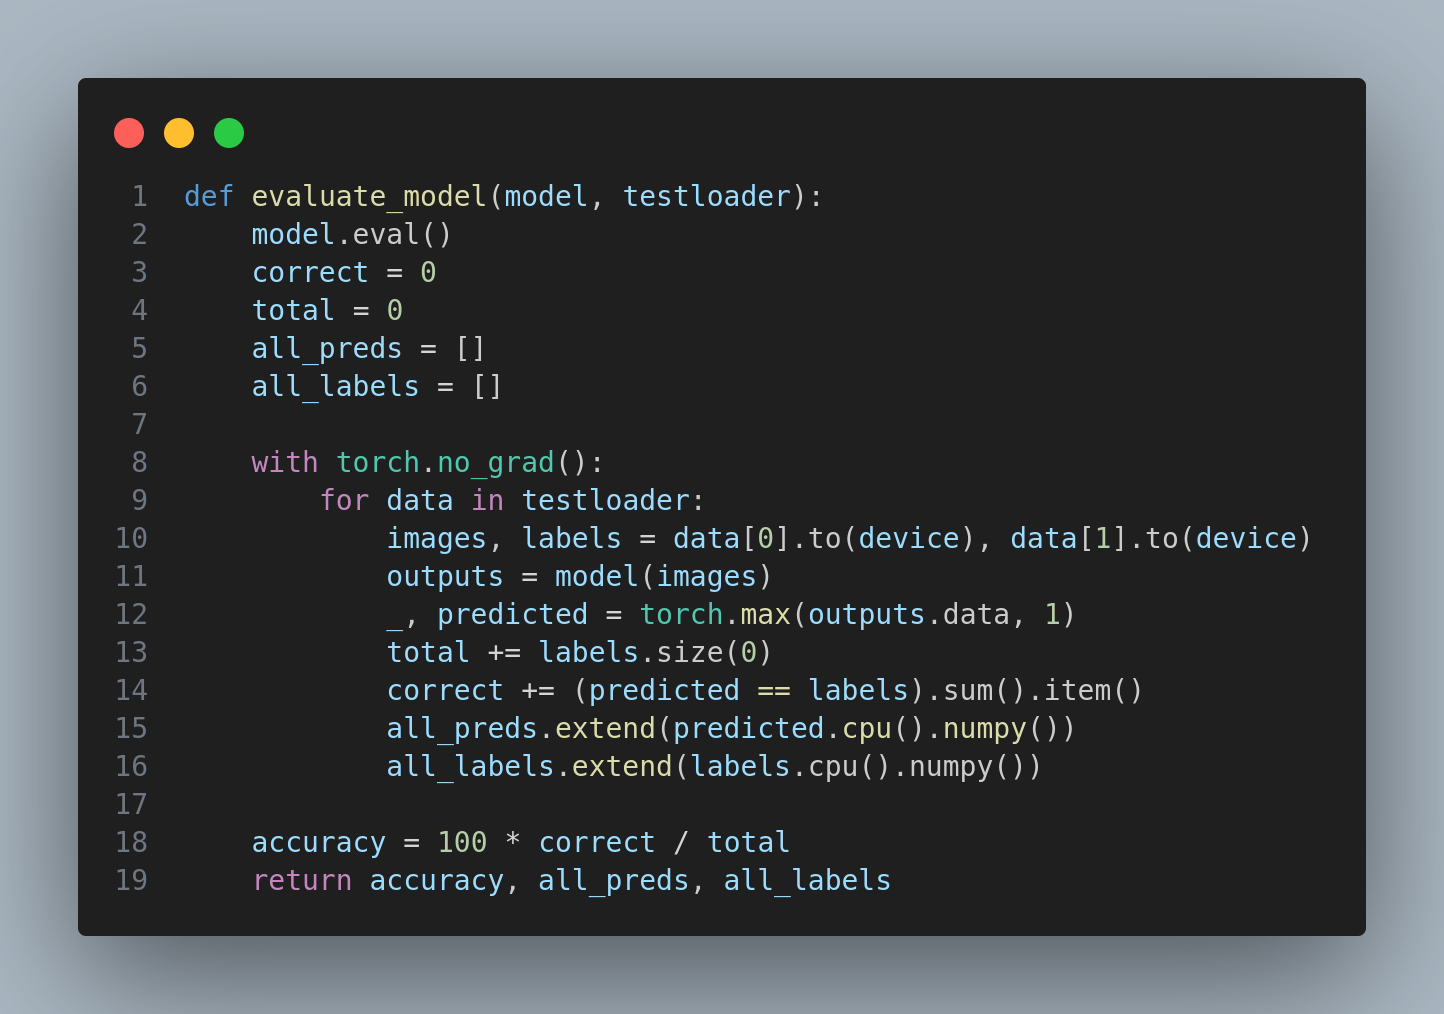
\includegraphics[width=0.7\linewidth]{images/evaluation_func.png}
    \caption{Evaluation function}
    \label{fig:enter-label}
\end{figure}

\begin{itemize}
    \item \textbf{Purpose}
    \begin{itemize}
        \item The \verb|evaluate_model| function is designed to assess the performance of a trained neural network model, such as a multilayer perceptron (MLP) or a convolutional neural network (CNN), on the CIFAR-10 test dataset. This function is crucial for understanding how well the model generalizes to new, unseen data after training. Specifically, it computes the test accuracy — the percentage of correct predictions — and also gathers the predicted and true class labels. These outputs are essential for quantitative evaluation and can also be used for additional analyses, such as building a confusion matrix or plotting precision-recall curves.
    \end{itemize}

    \item \textbf{Input(Arguments)}
    \begin{itemize}
        \item The function takes two arguments. The first is \verb|model|, which refers to a neural network that has already been trained. This model is a subclass of PyTorch’s \verb|nn.Module|, and it may be either an MLP or a CNN architecture specifically designed for image classification tasks. 
        
        \item The second input, \verb|testloader|, is a PyTorch \verb|DataLoader| object that provides batches of data from the CIFAR-10 test set. This dataset includes 10,000 labeled images divided into 10 classes, with images typically grouped into batches of 64 for efficient processing.
    \end{itemize}

    \item \textbf{Evaluation process}
    \begin{itemize}
        \item The evaluation begins with some initial setup. Two counters, \verb|correct| and \verb|total|, are initialized to zero to keep track of how many predictions are correct and the total number of samples evaluated. Additionally, two lists — \verb|all_preds| and \verb|all_labels| — are created to store the predicted class labels and the true class labels for all test samples. These lists are useful for downstream analysis like generating a confusion matrix or visualizing classification performance per class.

        \item The model is then set to evaluation mode using \verb|model.eval()|. This step is important because it ensures that any layers that behave differently during training and inference — such as dropout or batch normalization — are properly adjusted. Even though this specific model may not use such layers, it is good practice to always switch modes appropriately. To further optimize performance during inference, gradient tracking is disabled using with \verb|torch.no_grad()|. This ensures that PyTorch does not build the computational graph for backpropagation, reducing memory usage and speeding up computation.
        
        \item Within this no-gradient context, the function iterates over the test dataset in batches using a for loop. For each batch, the images and labels are moved to the appropriate device (CPU or GPU), depending on where the model is located. The images are passed through the model, which outputs a set of raw logits — unnormalized scores for each class. The predicted class for each image is then determined by selecting the index of the highest score using \verb|torch.max|. These predictions are compared with the true labels to determine how many are correct. The count of correct predictions is accumulated in \verb|correct|, and the total number of processed images is updated in \verb|total|. Simultaneously, the predicted and true labels are converted to NumPy arrays (moved to the CPU if necessary) and stored in their respective lists.
    \end{itemize}
\end{itemize}

The code lacks an explicit validation phase (e.g., a separate validation set). However, the training accuracy from \textbf{train\_model} serves as a proxy for monitoring performance during training. A true validation phase would require splitting the training set or modifying \textbf{train\_model} to evaluate on a validation \textbf{DataLoader}.

\subsection{Plot learning curves}

\begin{figure}[h]
    \centering
    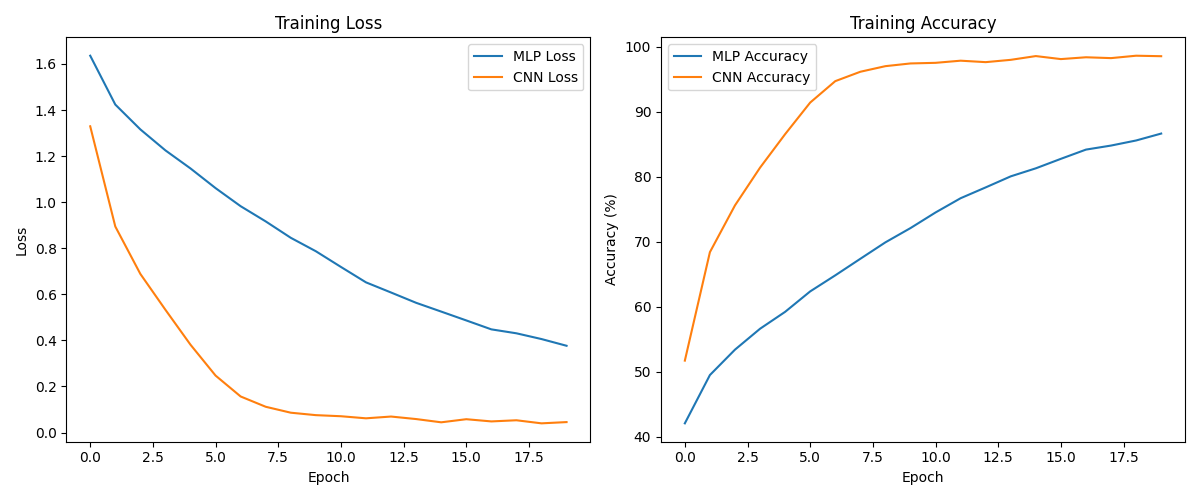
\includegraphics[width=0.8\linewidth]{images/learning_curves.png}
    \caption{Learning curves}
    \label{fig:enter-label}
\end{figure}
\newpage

\begin{enumerate}
    \item \textbf{Training loss}
    \begin{itemize}
        \item MLP loss (blue):
        \begin{itemize}
            \item Starts at ~1.6 and decreases steadily to ~0.4 by epoch 18.
            
            \item Shows a sharp initial drop, followed by a gradual decline, indicating the model learns quickly at first but slows as it approaches a local minimum.
        \end{itemize}

        \item CNN loss (orange):
        \begin{itemize}
            \item Starts at ~1.4 and drops more rapidly to ~0.2 by epoch 18.
            
            \item Demonstrates a steeper initial decrease and lower final loss, suggesting better convergence and a more effective feature extraction process.
        \end{itemize}

        \item Comparasion:
        \begin{itemize}
            \item The CNN consistently achieves a lower loss than the MLP, reflecting its superior ability to model the spatial structure of CIFAR-10 images.
            
            \item The gap widens after ~5 epochs, highlighting the CNN's advantage with deeper training.
        \end{itemize}

    \end{itemize}

    \item \textbf{Training accuracy}
    \begin{itemize}
        \item MLP loss (blue):
        \begin{itemize}
            \item Begins at ~40\% and rises steadily to ~75\% by epoch 18.
            
            \item Shows a moderate increase, with a noticeable plateau around 70-75\% after epoch 15, indicating limited learning capacity.
        \end{itemize}

        \item CNN loss (orange):
        \begin{itemize}
            \item Starts at ~50\% and increases more sharply to ~90\% by epoch 18.
            
            \item Exhibits a steep rise initially, followed by a gradual approach to a plateau near 90\%, suggesting strong learning and potential for further improvement with more epochs.
        \end{itemize}

        \item Comparasion:
        \begin{itemize}
            \item The CNN outperforms the MLP significantly, reaching ~90\% accuracy compared to ~75\% for the MLP.
            
            \item The CNN's higher accuracy aligns with its lower loss, confirming its effectiveness for image classification tasks like CIFAR-10.
        \end{itemize}
    \end{itemize}
\end{enumerate}
\newpage

\subsection{Plot confusion matrix}

\begin{figure}[h]
    \centering
    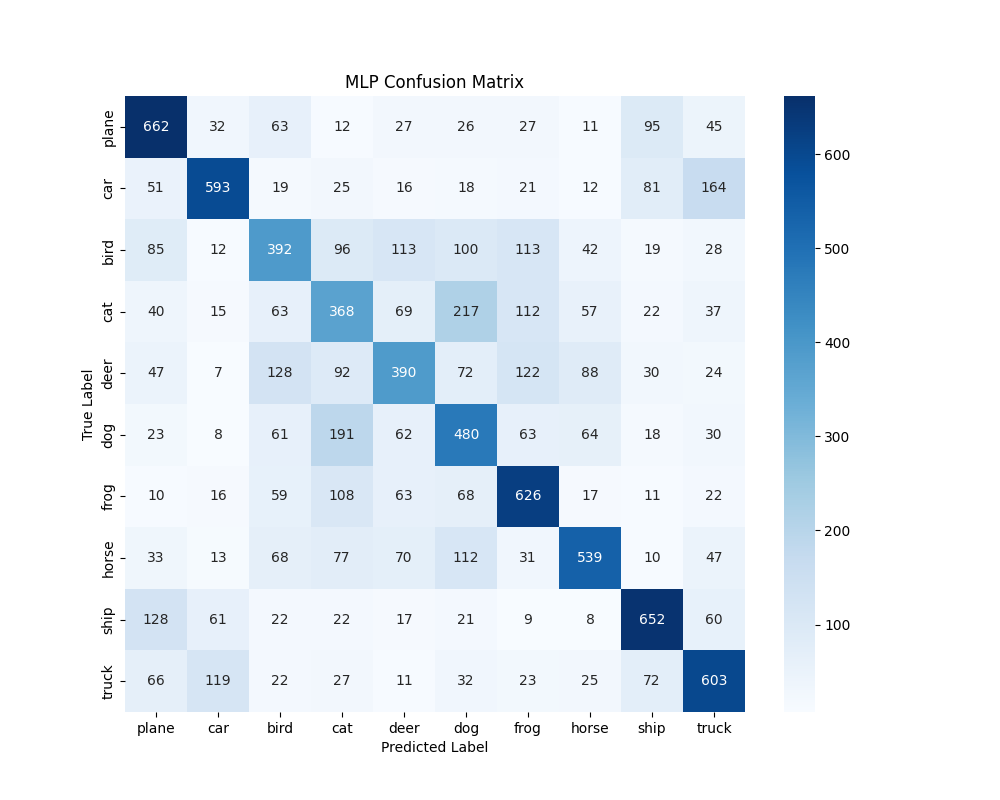
\includegraphics[width=0.9\linewidth]{images/mlp_confusion_matrix.png}
    \caption{MLP confusion matrix}
    \label{fig:enter-label}
\end{figure}

\begin{itemize}
    \item The MLP confusion matrix, created by the plot\_confusion\_matrix function, evaluates the model’s performance on the CIFAR-10 test set (10,000 images across 10 classes). The matrix shows ~71\% accuracy, with ~7,100 correct predictions (e.g., plane: 682, car: 593, frog: 626). Classes like frog (626), horse (539), and truck (603) have moderate accuracy (50-60\%), while cat (368) and dog (480) struggle, often confused with each other (191, 62) and deer (92, 72). Bird (392) also faces errors, misclassified as cat (96) and dog (100), due to visual similarities. 
    
    \item The MLP performs better on distinct classes (e.g., frog vs. truck) but struggles with similar ones, reflecting its limitation with flattened inputs. A validation set could help identify these issues earlier. This matrix aligns with the learning curves, showing the MLP’s weaker performance compared to the CNN.
\end{itemize}
\newpage

\begin{figure}[h]
    \centering
    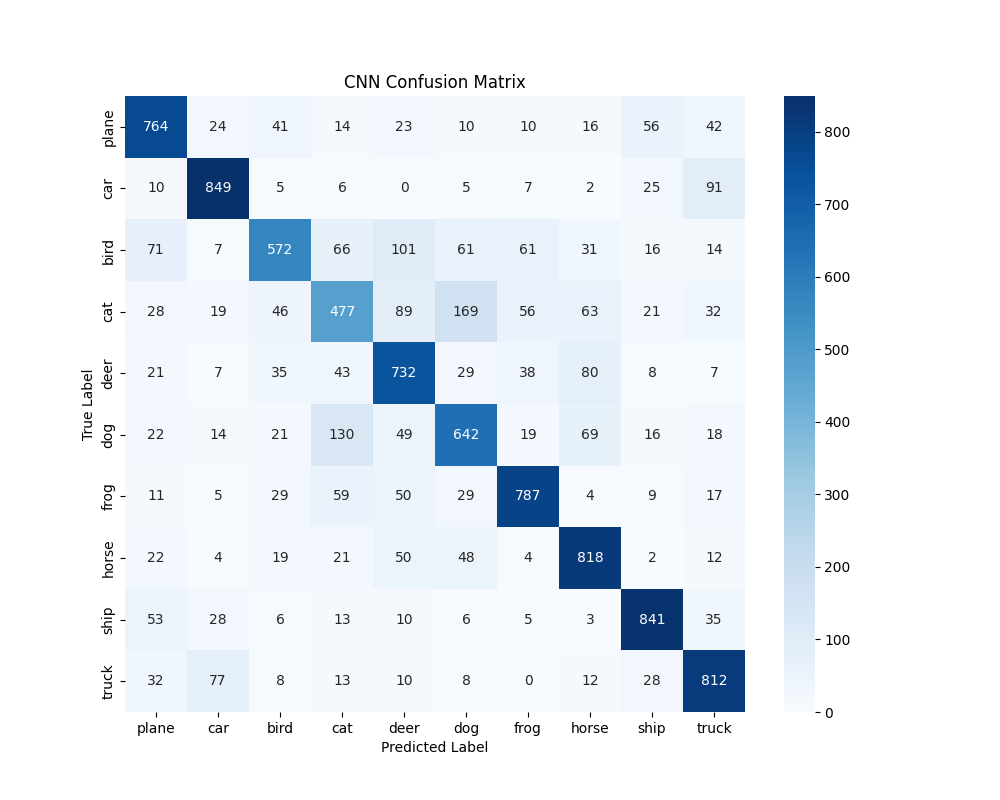
\includegraphics[width=0.9\linewidth]{images/cnn_confusion_matrix.png}
    \caption{CNN confusion matrix}
    \label{fig:enter-label}
\end{figure}

\begin{itemize}
    \item The CNN confusion matrix, generated by the plot\_confusion\_matrix function, evaluates the model’s performance on the CIFAR-10 test set (10,000 images across 10 classes). The matrix shows ~90\% accuracy, with ~9,000 correct predictions (e.g., car: 849, frog: 787, horse: 818). High-accuracy classes like car and ship exceed 80\%, while dog (642) struggles, often confused with cat (130) and deer (49). Bird (572) and cat (477) also face errors, misclassified with plane (71) and dog (130), respectively, due to visual similarities. 
    
    \item The CNN excels at distinguishing dissimilar classes (e.g., frog vs. truck) but needs improvement for similar ones. A validation set could help address these issues earlier. This matrix complements the learning curves, highlighting the CNN’s strengths and weaknesses.
\end{itemize}
\newpage

\subsection{Compare and discuss the results of the two neural networks}

\begin{figure}[h]
    \centering
    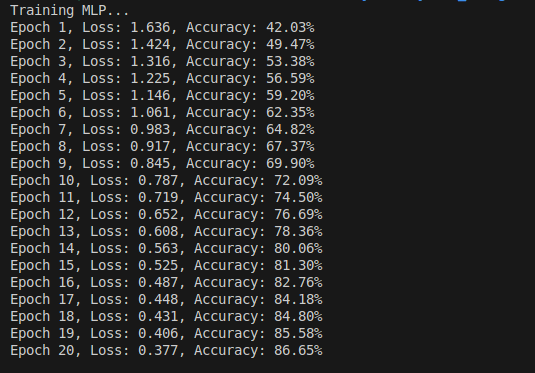
\includegraphics[width=0.6\linewidth]{images/MLP_train.png}
    \caption{MLP train results}
    \label{fig:enter-label}
\end{figure}

\begin{itemize}
    \item The MLP was trained on the CIFAR-10 dataset for 20 epochs, starting with a loss of 1.636 and 42.03\% accuracy in epoch 1, as shown in the training log. By epoch 20, its loss decreased to 0.377, and training accuracy rose to 86.65\%, reflecting steady learning progress. However, the test accuracy, reported at 53.05\%, reveals a significant gap from the training accuracy, indicating likely overfitting. 
    
    \item The MLP’s performance plateaus after ~15 epochs, with diminishing gains in accuracy, suggesting its limited capacity to generalize on image data due to the lack of spatial feature extraction. Incorporating a validation set during training could help detect and mitigate this overfitting earlier, improving model selection.
\end{itemize}

\begin{figure}[h]
    \centering
    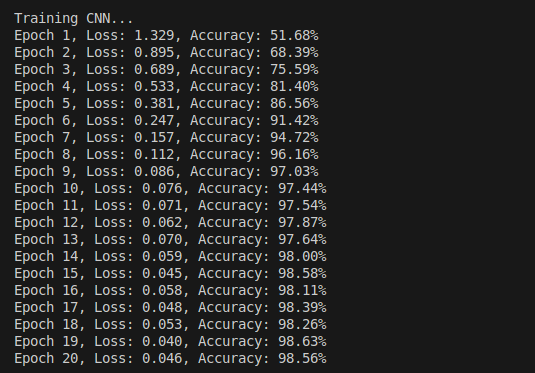
\includegraphics[width=0.6\linewidth]{images/CNN_train.png}
    \caption{CNN train results}
    \label{fig:enter-label}
\end{figure}

\begin{itemize}
    \item The CNN was trained on the CIFAR-10 dataset for 20 epochs, beginning with a loss of 1.329 and 51.68\% accuracy in epoch 1, according to the training log. By epoch 20, its loss dropped sharply to 0.046, and training accuracy reached 98.56\%, demonstrating rapid and effective learning. The test accuracy of 72.94\% is notably lower than the training accuracy, suggesting some overfitting, though less severe than the MLP’s.
    
    \item The CNN’s steep improvement and higher accuracy reflect its ability to capture spatial features in images, making it more suitable for CIFAR-10. Adding a validation set could further optimize training by identifying overfitting early and refining the model’s generalization.\
\end{itemize}

\begin{figure}
    \centering
    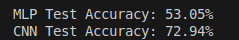
\includegraphics[width=0.5\linewidth]{images/result.png}
    \caption{Comparison}
    \label{fig:enter-label}
\end{figure}

\begin{itemize}
    \item The image shows the test accuracy results for two models: MLP with 53.05\% accuracy and CNN with 72.94\% accuracy. From this we can conclude that The CNN (Convolutional Neural Network) likely outperforms the MLP (Multi-Layer Perceptron) because CNNs are specifically designed for image data. They use convolutional layers to automatically detect spatial patterns and features, reducing the need for manual feature engineering. MLPs, being fully connected networks, struggle with high-dimensional data like images and are more prone to overfitting without such specialized architecture.
\end{itemize}


\end{document}